\section{Tipos de aprendizado}

Os sistemas de aprendizado de máquina possuem características peculiares que possibilitam uma classificação não exclusiva desses sistemas em função da linguagem de descrição, modo de aprendizado, paradigma de aprendizado, formas e tarefa de aprendizado.
O aprendizado depende da interação entre o ambiente e aprendiz. A primeira diferença consiste no aprendizado supervisionado e não supervisionado \cite{uml}.

\subsection{Aprendizado supervisionado}

O aprendizado supervisionado é aquele cujos parâmetros são pré-definidos e o algoritmo procura um padrão entre os dados. As informações que serão utilizadas para treinamento já contêm informações suficientes que permitem o algoritmo inferir uma relação entre uma ou múltiplas variáveis. A característica básica de sistemas de aprendizado supervisionado é de que os dados que são utilizados para treiná-los contém a resposta desejada, isto é, contém a variável dependente resultante das variáveis independentes observadas. Nesse caso, alega-se que os dados são anotados com as respostas ou classes a serem previstas \cite{learning-algorithms}.

De acordo com \citeonline{learning-algorithms} as técnicas mais usuais para resolver problemas de aprendizado supervisionado são: regressão linear, regressão logística, redes neurais artificiais, máquina de suporte vetorial (ou máquinas kernel), árvores de decisão, k-vizinhos mais próximos e Bayes ingênuo. Aprendizado de máquina supervisionado é a área que concentra a maioria das aplicações bem sucedidas e onde a grande parte dos problemas já estão bem definidos.

A Figura \ref{fig:reg-linear} representa um exemplo de aprendizado supervisionado, a regressão linear.

\begin{figure}[h]
    \caption{Regressão linear é um exemplo de aprendizado supervisionado}
    \centering
    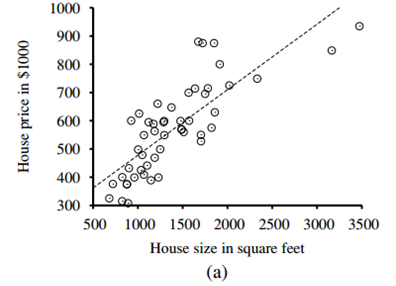
\includegraphics[width=0.8\textwidth]{Textuais/Figuras/linear-ml.png}
    \fonte{\citeonline{ai}}
    \label{fig:reg-linear}
\end{figure}

\subsection{Aprendizado não-supervisionado}

O aprendizado não supervisionado, permite abordar problemas com pouca ou nenhuma ideia de como deverá ser o resultado. A rede tem de descobrir relações, padrões, regularidades ou categorias nos dados que lhe vão sendo apresentados e codificá-las em saídas. Em alguns casos, conseguir dados anotados é extremamente custoso ou até mesmo impossível. De uma forma geral, com aprendizado não supervisionado pretende-se achar uma representação mais informativa dos dados que temos. Geralmente, essa representação mais informativa é também mais simples, condensando a informação em pontos mais relevantes \cite{ai}.

A Figura \ref{fig:nao-supervisionado} exemplifica o aprendizado não supervisionado: a classificação de dados em dois grupos.

\begin{figure}[h]
    \caption{(a) Distribuição da altura e peso de algumas pessoas. (b) Possível agrupamento de dados em 2 grupos}
    \centering
    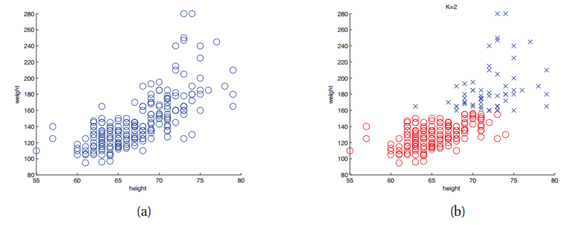
\includegraphics[width=1.0\textwidth]{Textuais/Figuras/nao-supervisionado.png}
    \fonte{Murphy (2012)}
    \label{fig:nao-supervisionado}
\end{figure}

\subsection{Benefícios das RNA}

O poder de abstração das RNA deve-se à sua estrutura paralela e à capacidade de aprendizagem \cite{big-data}. A estrutura paralela resulta da existência de muitos neurônios ligados em uma mesma estrutura de pesos de conexão com facilidade de adaptação a distintos tipos de entrada de dados. A estrutura paralela é desejável uma vez que permite a tolerância à falha, pois se algum neurônio falhar, os efeitos na rede como um todo não serão significativos para o desempenho da rede, dado que existe outro caminho de ligação entre os nós que pode iludir a falha \cite{statistical-learning}.

Uma das principais características das RNA é a capacidade de aprender por meio de exemplos e de generalização, ou seja, reconhecer padrões em elementos que não foram apresentados antes, possibilitando a produção de resultado aceitável oriundo de uma nova entrada de informação \cite{neural-network}.

As principais propriedades que podem se destacar das redes neurais artificiais são: não linearidade, mapeamento de entrada e saída, adaptabilidade e tolerância a falhas \cite{neural-network}.

\subsection{Redes Neurais Artificiais}

Redes neurais artificiais foram originalmente planejadas no meio do século 20 como um modelo computacional do cérebro humano. Sua aplicação era limitada devido a limitação computacional disponível na época, além de algumas questões teóricas que não foram solucionadas por várias décadas \cite{mlpp}.

É teorizado que devido à sua inspiração biológica, algoritmos baseados em redes neurais artificiais serão capazes de simular como o ser humano reconhece conceitos e objetos \cite{learning-algorithms}.

Em uma análise matemática, as RNA podem ser explicadas como um mapeamento não linear de um vetor de espaço de entrada para um vetor de espaço de saída, que pode ser realizado por meio de camadas de funções de ativação, em que coordenadas de entrada são somadas de acordo com o valor de seus respectivos pesos e bias  para produzir uma saída simples, ativada ou não, de acordo com o respectivo nível de acionamento \cite{two-phase-flow}.

O conceito de rede neural artificial é basicamente introduzido pela biologia onde a rede neural tem um importante papel no ser humano. No corpo humano todo trabalho é realizado com ajuda da rede neural. Uma rede neural é uma cadeia de milhões de neurônios interconectados \cite{ann}, exemplificado pela Figura \ref{fig:neuronios}.

\begin{figure}[h]
    \caption{Neurônios humanos conectados entre si}
    \centering
    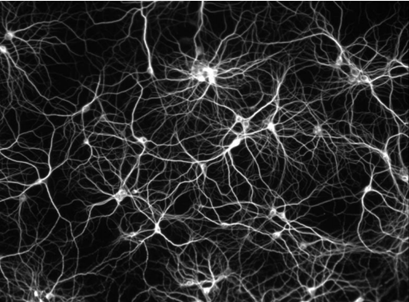
\includegraphics[width=0.55\textwidth]{Textuais/Figuras/neuronios.png}
    \fonte{Autores}
    \label{fig:neuronios}
\end{figure}

A terminologia rede neural é inspirada pelas operações biológicas realizadas por células especiais denominadas neurônios, mostrados na Figura \ref{fig:celula}. Um neurônio é uma célula biológica especial que processa informação de um neurônio para outro com ajuda de um impulso elétrico e mudanças químicas que ocorrem no cérebro. Todo o processo de receber e enviar informação é realizado de uma forma particular: um neurônio recebe informações de outro neurônio através dos dendritos e envia informações com picos de atividade elétrica através de um longo e fino suporte conhecido como axônio que os divide em sinapses para enviá-los para outros neurônios \cite{ai}.

\begin{figure}[h]
    \caption{Nomenclatura das partes que compõem um neurônio humano}
    \centering
    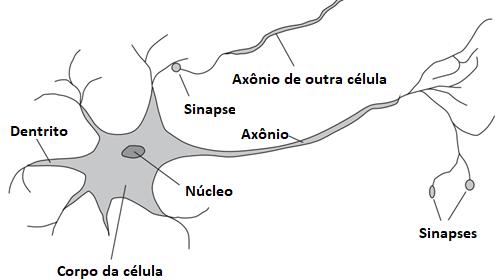
\includegraphics[width=0.8\textwidth]{Textuais/Figuras/celula.png}
    \fonte{https://news.psu.edu/story/441320/2016/12/08/research/how-make-motor-neuron}
    \label{fig:celula}
\end{figure}

As redes neurais artificiais têm o seu equivalente ao neurônio denominado nó que recebe um conjunto de entradas ponderadas, processa a sua soma com as funções de ativação $\phi$, e passa o resultado da função de ativação para o próximo nó até o término da rede (Equação \ref{eq:no}) \cite{ann}.

\begin{equation}
\label{eq:no}
    \phi \left( \sum_{i} w_i\times a_i \right) = \phi(w^T\times a)
\end{equation}

Visualmente é equivalente a Figura \ref{fig:neuronio-rna}.

\begin{figure}[h]
    \caption{Representação de um neurônio na RNA}
    \centering
    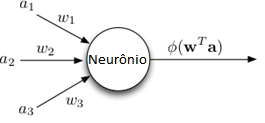
\includegraphics[width=0.31\textwidth]{Textuais/Figuras/rep-neronio.png}
    \fonte{http://briandolhansky.com/blog/artificial-neural-networks-linear-regression-part-1}
    \label{fig:neuronio-rna}
\end{figure}

\subsection{Funções de ativação}

Funções de ativação são basicamente funções de transferência que são geradas pelos neurônios artificiais e enviam sinais para outro neurônio artificial \cite{ann}. As funções de ativação mais comuns são: Limiar, Degrau, Degrau Unitário, Linear e Logística. A Figura \ref{fig:funcao-ativacao} ilustra essas funções. 

\begin{figure}[h]
    \caption{Funções de ativação}
    \centering
    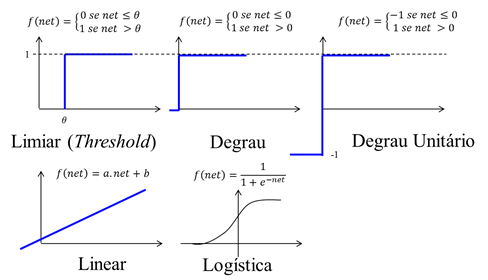
\includegraphics[width=0.8\textwidth]{Textuais/Figuras/funcao-ativacao.png}
    \fonte{https://pt.stackoverflow.com/questions/61187/como-implementar-a-camada-oculta-em-uma-rede-neural-de-reconhecimento-de-caracte}
    \label{fig:funcao-ativacao}
\end{figure}

A função de ativação linear é a função mais básica porque não altera a saída de um neurônio. Geralmente é utilizada nas camadas de saída em redes neurais de regressão. A Equação \ref{eq:linear}, mostra a função linear que também é denominada função identidade \cite{ai}.

\begin{equation}
\label{eq:linear}
    \phi(w^Ta) =w^Ta
\end{equation}

A função sigmoide (Logística) era a mais utilizada em RNAs, por serem biologicamente mais plausíveis. Como neurônios biológicos funcionam de forma binária (ativando vs não ativando), a função sigmoide é uma boa forma de modelar esse comportamento, já que assume valores apenas entre 0 (não ativação) e 1 (ativação). No entanto, observando sua derivada, pode-se ver que ela satura para valores acima de 5 e abaixo de -5. Com essas derivadas tendendo a zero, a propagação do gradiente desvanece nessas regiões, causando dificuldades no treinamento. A função logística é representada pela Equação \ref{eq:sigmoid} \cite{ai}.

\begin{equation}
\label{eq:sigmoid}
    \phi(w^Ta)=\frac{1}{1+exp(-w^Ta)} 
\end{equation}

Similar à função logística, a função Tangente Hiperbólica (tanh) também tem um formato de S, mas varia de -1 a 1, em vez de 0 a 1 como na logística. A tanh se aproxima mais da identidade, sendo assim uma alternativa mais atraente do que a sigmoide para servir de ativação às camadas ocultas das RNAs \cite{ai}.

\begin{equation}
\label{eq:tanh}
    \phi(w^Ta) = tanh(w^Ta)
\end{equation}

A possível criação de uma rede neural ocorre por meio do encadeamento dos nós. Usualmente esse processo é realizado utilizando camadas, as saídas de um nó estão conectadas a entrada dos nós da próxima camada \cite{tensor-flow}.

O objetivo de aproximações de funções é treinar uma rede neural que seja capaz, a partir de um conjunto de dados entrada-saída, de mapear uma determinada relação funcional que contemple o universo de amostras sob análise. O treinamento, nesse caso, envolve o aprendizado dos pesos de borda corretos para produzir a saída de destino, dada uma entrada \cite{uml}. A rede e seus pesos treinados formam uma função (denominada h) que operam sob dados de entrada. Com a rede treinada, é possível produzir previsões para valores de entrada previamente desconhecidos.

\begin{figure}[h]
    \caption{Exemplo de uma regressão e classificação}
    \centering
    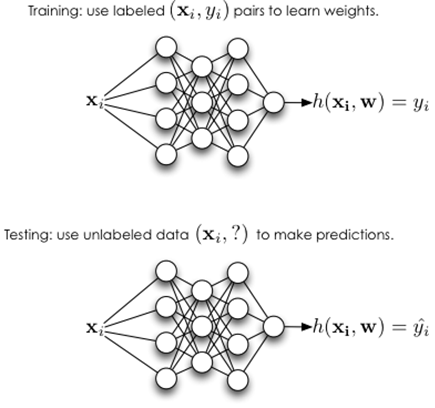
\includegraphics[width=0.7\textwidth]{Textuais/Figuras/rede-neural.png}
    \fonte{https://towardsdatascience.com/how-to-build-your-own-neural-network-from-scratch-in-python-68998a08e4f6}
    \label{fig:reg-class}
\end{figure}

É possível treinar uma rede neural para realizar regressão ou classificação. Nesse trabalho iremos abordar somente a regressão linear. 

\subsection{Regressão Linear}

Regressão linear é a forma mais simples de regressão \cite{ai}. Modelam-se o sistema como combinações lineares de entradas para produzir uma saída.

\begin{equation}
    y_i = h(x_i,w) = w^Tx_i
\end{equation}

A RNA torna-se responsável por encontrar os pesos que geram o melhor resultado para os dados de treinamento. Um modo de verificar a qualidade da aproximação é utilizando o método dos mínimos quadrados (também conhecido como \textit{Loss}) \cite{ltflow}.

\begin{equation}
    L(w) = \sum_i \left( h(x_i,w)-y_i^2 \right)^2
\end{equation}

Para poder realizar o melhor ajuste é preciso minimizar o valor de $L(w)$. Esse método possui uma solução analítica, mas em geral pode-se resolver utilizando o método do gradiente descendente \cite{ai}.

A rede neural mais simples utiliza o método dos mínimos quadrados para realizar uma regressão linear como mostra a Figura \ref{fig:linear}. 

\begin{figure}[h]
    \caption{Neurônio artificial e a saída gerada utilizando uma função linear de ativação}
    \centering
    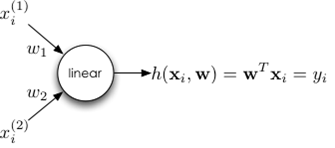
\includegraphics[width=0.45\textwidth]{Textuais/Figuras/linear.png}
    \fonte{http://briandolhansky.com/blog/artificial-neural-networks-linear-regression-part-1}
    \label{fig:linear}
\end{figure}

Essa rede recebe como entrada de dados, duas entradas $x_i^{(1)}$ e $x_i^{(2)}$, os pesos das entradas como $w_1$ e $w_2$ e os soma, e como saída tem-se a previsão $y_i$. Pode-se considerar uma rede neural com n parâmetros de entrada, porém a rede deve conter n pesos, sendo equivalente um peso para cada entrada. Para poder determinar a qualidade de aproximação é possível utilizar o método dos mínimos quadrados \cite{ML}.

\citeonline{tensor-flow} utiliza o método do gradiente descendente para minimizar os erros em relação aos dados de treinamento. Primeiramente deriva-se o gradiente descendente em relação a um determinado peso $w_{j \rightarrow k}$

\begin{equation}
    \frac{\partial}{\partial w_{j \rightarrow k}}L(w) = \frac{\partial}{\partial w_{j \rightarrow k}} \sum_i \left( h(x_i,w)-y_i^2 \right)
\end{equation}

\begin{equation}
    \frac{\partial}{\partial w_{j \rightarrow k}}L(w) = \sum_i \frac{\partial}{\partial w_{j \rightarrow k}} \left( h(x_i,w)-y_i^2 \right)
\end{equation}

\begin{equation}
    \frac{\partial}{\partial w_{j \rightarrow k}}L(w) = \sum_i 2(h(x_i,w)-y_i) \frac{\partial}{\partial w_{j \rightarrow k}} h(x_i,w)
\end{equation}

Nesse ponto, calcula-se o gradiente da função da rede em relação ao peso da derivada parcial. 

A função da rede é dada pela Equação \ref{eq:funcao-rede}.

\begin{equation}
\label{eq:funcao-rede}
    h(x_i,w) = w_1x_i^{(1)} + w_2x_i^{(2)}
\end{equation}

O gradiente em relação a $w_1$ é apenas $x_1$, e o gradiente em relação a $w_2$ é apenas $x_2$, dessa forma o gradiente é dado pela Equação \ref{eq:gradiente}.

\begin{equation}
\label{eq:gradiente}
    \nabla_wL(w) = \left( \frac{\partial L(w)}{\partial w_1}, \frac{\partial L(w)}{\partial w_2} \right) = \left( \sum_i 2x_i ^{(1)} h(x_i,w), \sum_i 2x_i ^{(2)} h(x_i,w) \right)
\end{equation}

Agora é possível atualizar os pesos utilizando o gradiente descendente padrão

\begin{equation}
    w = w -\eta \nabla_w L(w)
\end{equation}

Onde ``$\eta$`` é o passo.

\subsection{Treinamento da RNA}

Nesta fase, seguindo o algoritmo de treinamento escolhido, serão ajustados os pesos das conexões. É importante considerar, nesta fase, alguns aspectos tais como a inicialização da rede, o modo de treinamento e o tempo de treinamento \cite{aplicacao}.

Uma boa escolha dos valores iniciais dos pesos da rede pode diminuir o tempo necessário para o treinamento. Normalmente, os valores iniciais dos pesos da rede são números aleatórios uniformemente distribuídos, em um intervalo definido. A escolha errada destes pesos pode levar a uma saturação prematura. \citeonline{treinamento} encontraram uma função que pode ser utilizada para determinar valores iniciais melhores que valores puramente aleatórios \cite{aplicacao}.

Quanto ao modo de treinamento, na prática é mais utilizado o modo padrão devido ao menor armazenamento de dados, além de ser menos suscetível ao problema de mínimos locais, devido à pesquisa de natureza estocástica que realiza. Por outro lado, no modo batch se tem uma melhor estimativa do vetor gradiente, o que torna o treinamento mais estável. A eficiência relativa dos dois modos de treinamento depende do problema que está sendo tratado \cite{aplicacao}.

Quanto ao tempo de treinamento, vários fatores podem influenciar a sua duração, porém sempre será necessário utilizar algum critério de parada. O critério de parada do algoritmo recorrente não é bem definido, e geralmente é utilizado um número máximo de ciclos. Mas, devem ser considerados a taxa de erro médio por ciclo, e a capacidade de generalização da rede. Pode ocorrer que em um determinado instante do treinamento a generalização comece a degenerar, causando o problema de \textit{over-training}, ou seja a rede se especializa no conjunto de dados do treinamento e perde a capacidade de generalização \cite{aplicacao}.

O treinamento deve ser interrompido quando a rede apresentar uma boa capacidade de generalização e quando a taxa de erro for suficientemente pequena, ou seja menor que um erro admissível. Assim, deve-se encontrar um ponto ótimo de parada com erro mínimo e capacidade de generalização máxima \cite{aplicacao}.

\subsection{Testando a RNA}

Durante esta fase o conjunto de teste é utilizado para determinar a performance da rede com dados que não foram previamente utilizados. A performance da rede, medida nesta fase, é uma boa indicação de sua performance real.

Devem ser considerados ainda outros testes como análise do comportamento da rede utilizando entradas especiais e análise dos pesos atuais da rede, pois se existirem valores muito pequenos, as conexões associadas podem ser consideradas insignificantes e assim serem eliminadas (\textit{prunning}). De modo inverso, valores substantivamente maiores que os outros poderiam indicar que houve \textit{over-training} da rede.

Com a rede treinada, testar consiste em obter a previsão para cada ponto $x_i$ utilizando a função $h(x_i, w)$. O erro pode ser calculado da mesma forma do treinamento utilizando a Equação \ref{eq:teste-rna}.

\begin{equation}
\label{eq:teste-rna}
    L(w) = (\overline{y_i} - y_i)^2
\end{equation}

\subsection{Redes Neurais Recorrentes}

Diferentemente das redes neurais \textit{feed-forward}, redes neurais recorrentes possuem ciclos entre seus neurônios. Em outras palavras, neurônios podem ter conexões com neurônios de camadas anteriores, ou da mesma camada como mostra a Figura \ref{fig:recorrente}.

\begin{figure}[h]
    \caption{Exemplo de uma rede neural recorrente}
    \centering
    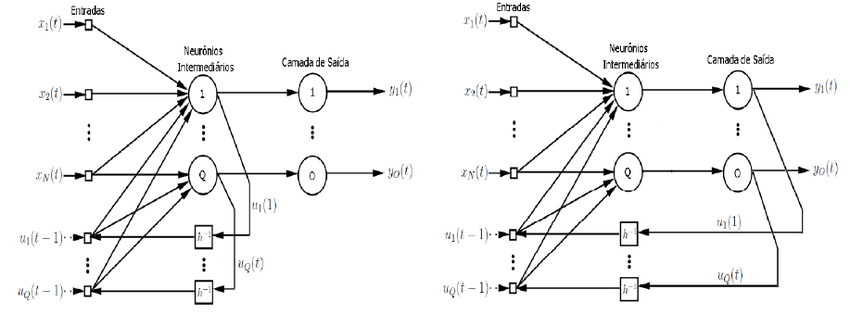
\includegraphics[width=0.9\textwidth]{Textuais/Figuras/recorrente.png}
    \fonte{https://goo.gl/wH6xmR}
    \label{fig:recorrente}
\end{figure}

Desta forma, a informação não flui em um único sentido, e a saída da rede não depende mais apenas da entrada corrente, mas também das entradas anteriores. O efeito prático disto é a existência de memória de curto prazo na rede.

Considerando o aprendizado por treinamento uma espécie de memória de longo prazo, então adicionalmente à nova capacidade de manter uma memória recente, redes neurais recorrentes podem criar modelos muito mais complexos, que apesar de serem de compreensão mais difícil apresentam capacidade de resolver uma gama maior de problemas \cite{rede-recorrente}.

Mesmo com redes neurais \textit{feed-forward} é possível ter um efeito similar ao de memória, como por exemplo, adicionando à entrada dados de entradas anteriores, multiplicando a dimensionalidade, ou mesmo adicionando parâmetros com algum aspecto temporal. Mas esses casos podem acabar causando o problema de maldição da dimensionalidade (\textit{curse of dimensionality}) onde a entrada fica muito complexa e dificulta o aprendizado e generalização \cite{rede-recorrente}.

Contudo, mesmo redes neurais recorrentes podem apresentar desafios no processo de treinamento. Ainda que na teoria sejam capazes de lidar com dependências de longo termo (longas sequências), Bengio et al. (1994) mostram através de experimentos que na prática isso muitas vezes não é possível, pois em métodos de treinamento baseados em gradientes a informação de erro desaparece \cite{rede-recorrente}.

\subsubsection{Limitações de redes recorrentes}

As redes neurais que utilizam recorrência, assim como muitos outros tipos de redes neurais artificiais, podem ser vistas como ``caixas pretas``, na qual quase não se sabe porque a rede chega a uma determinada saída, uma vez que os modelos não apresentam justificativas para suas respostas. Neste sentido, muitas pesquisas vêm sendo realizadas visando a extração de conhecimento de redes neurais artificiais, e na criação de procedimentos explicativos, onde se tenta justificar o comportamento da rede em determinadas situações  \cite{aplicacao}.

Uma outra limitação refere-se ao tempo de treinamento de redes neurais utilizando recorrência, que tende a ser muito lento. Algumas vezes são necessários milhares de ciclos para se chegar à níveis de erros aceitáveis, principalmente se estiver sendo simulado em computadores seriais, pois a CPU deve calcular as funções para cada unidade e suas conexões separadamente, o que pode ser problemático em redes muito grandes, ou com grande quantidade de dados \cite{aplicacao}.

É muito difícil definir a arquitetura ideal da rede de forma que ela seja tão grande quanto o necessário para conseguir obter as representações necessárias, ao mesmo tempo compacta o suficiente para se ter um treinamento mais acelerado. Não existem regras claras para se definir quantas unidades devem existir nas camadas ocultas, quantas camadas, ou como devem ser as conexões entre os neurônios artificiais. Para resolver este tipo de problema, Algoritmos Genéticos poderiam ser utilizados para encontrar automaticamente boas arquiteturas de redes neurais, eliminando muitas armadilhas associadas às abordagens de engenharia humana \cite{aplicacao}.
